\textbf{Question: Plot $g_\gamma(x)$ vs. $x$ in the range $x\in [-{\rm FS},{\rm FS}]$ for $\gamma = 0$, $1$ and $2$. For input signals whose values are always much smaller than $\rm FS$ (in absolute value), what will be the effect of the nonlinearity?
}
\vspace{0.5cm}

For inputs with amplitude much smaller than \(FS\), the nonlinearity \(g_{\gamma}(x)\) acts essentially as a constant gain: using $\lim_{\gamma \to 0} g_{\gamma}(x) = x$.
Thus, for \(|x|\ll FS\) the block only rescales the signal (no significant harmonic distortion) and the quantiser that follows sees an almost linearly amplified input. Significant compression and distortion appear only when \(|x|\) becomes a noticeable fraction of \(FS\).

\begin{figure}[H]
    \centering
    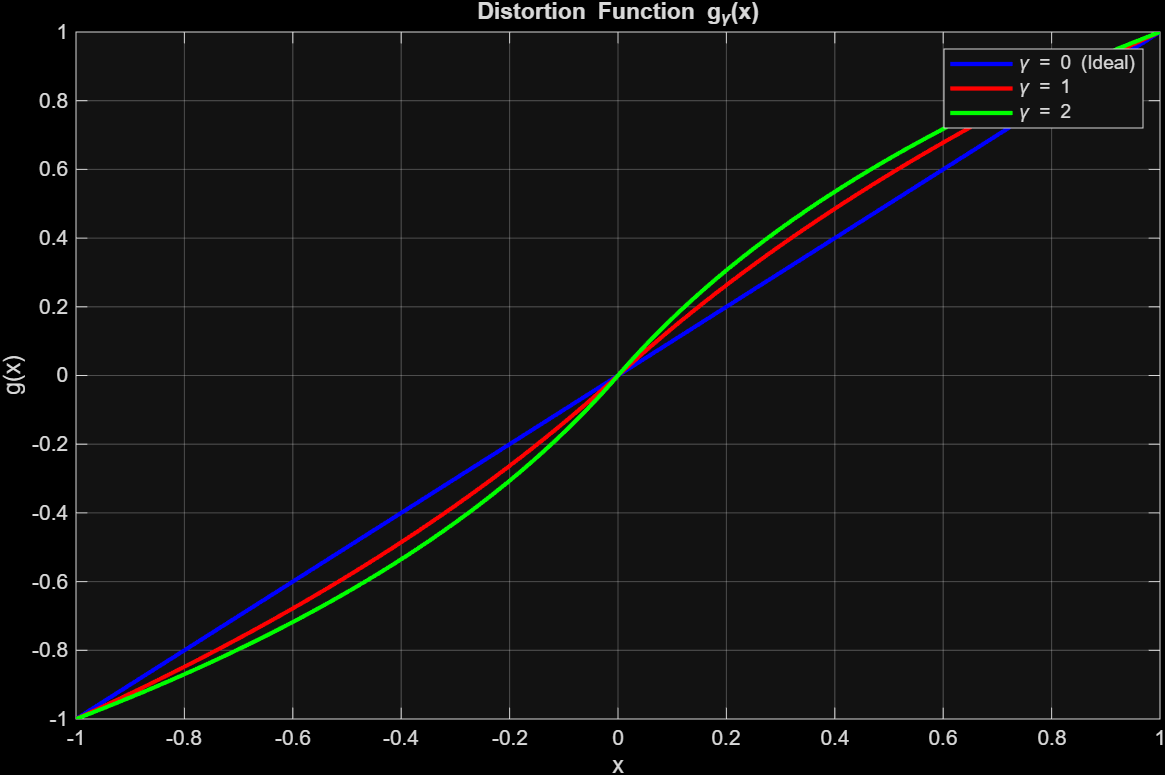
\includegraphics[width=1\textwidth]{img/task5_1.png}
    \label{fig:task5_1}
\end{figure}

\vspace{1cm}
\textbf{Question: Modify the code in {\tt quanti.m} and write a Matlab function {\tt dquanti.m} implementing this nonuniform quantizer. The format should be similar to that of {\tt quanti.m}, but including an additional input parameter {\tt gama}:}
\begin{center}
{\tt xq = dquanti( x, FS, Nbits, gama ); }
\end{center} 
\vspace{0.5cm}

We modified the function {\tt dquanti.m} as requested, if we receive \texttt{gama=0} the function behaves as a uniform quantizer, otherwise it applies the non-linear distortion before quantization.

The code is as follows:
\begin{lstlisting}[language=Matlab]
    function y = dquanti(x, FS, Nbits, gama)
    if gama == 0
        g_x = x; % Si gama=0, no hay distorsion (g(x) = x)
    else
        g_x = sign(x) .* (FS / log(1 + gama)) .* log(1 + gama .* abs(x) / FS);
        g_x(x == 0) = 0;
    end

    FS    = abs(FS);
    FSbin = 2^(Nbits-1);
    LSB   = FS/FSbin;  

        y = round(g_x/LSB); 
        y = min(y, FSbin-1); 
        y = max(y, -FSbin); 
        y = y * LSB;
\end{lstlisting}

\vspace{1cm}
\textbf{Question: Generate  samples (at 100 MHz) of a full-scale sinusoid with $f_0 = 6.8359$ MHz.
Quantize them to $N=11$ bits using $\gamma = 0.003$ in {\tt dquanti}. 
Determine the SFDR in dBFS using an FFT size $M=2048$, and then with $M=512$. 
Does the SFDR depend on the FFT size? Does the noise floor depend on the FFT size? How do you explain this?
}
\vspace{0.5cm}

We obtain the SFDR values from the FFT plots shown in Figures~\ref{fig:task5_2048} and~\ref{fig:task5_512}.
The SFDR values are:
\begin{itemize}
    \item For \(M=2048\): SFDR -71.3586 dBFS
    \item For \(M=512\): SFDR -71.2428 dBFS
\end{itemize}

For both $M=2048$ and $M=512$, the FFT of the quantized 11-bit sinusoid ($f_0=6.8359$\,MHz, $\gamma=0.003$) shows almost the same main harmonic and a largest spur.
Increasing the FFT size only reveals more detail in the lower part of the spectrum but does not change the SFDR value itself.

\begin{figure}[H]
    \centering
    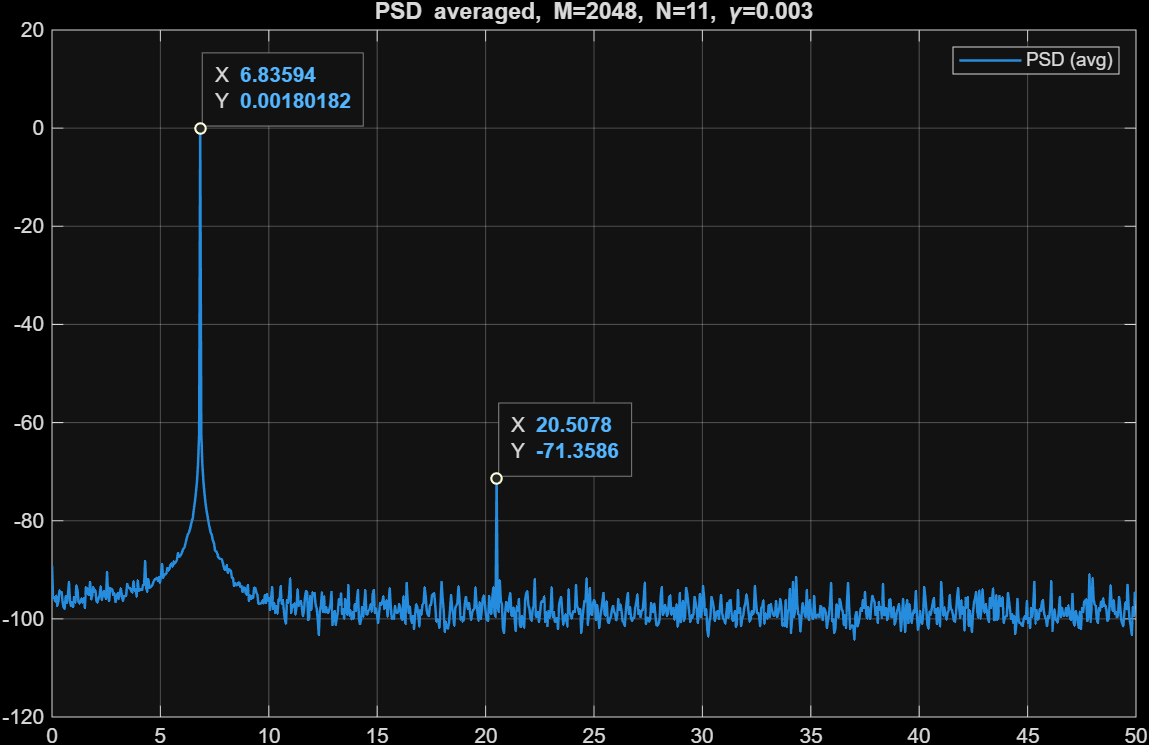
\includegraphics[width=1\textwidth]{img/task5_2048.png}
    \caption{FFT with $M=2048$, $N=11$, $\gamma=0.003$}
    \label{fig:task5_2048}
\end{figure}

\begin{figure}[H]
    \centering
    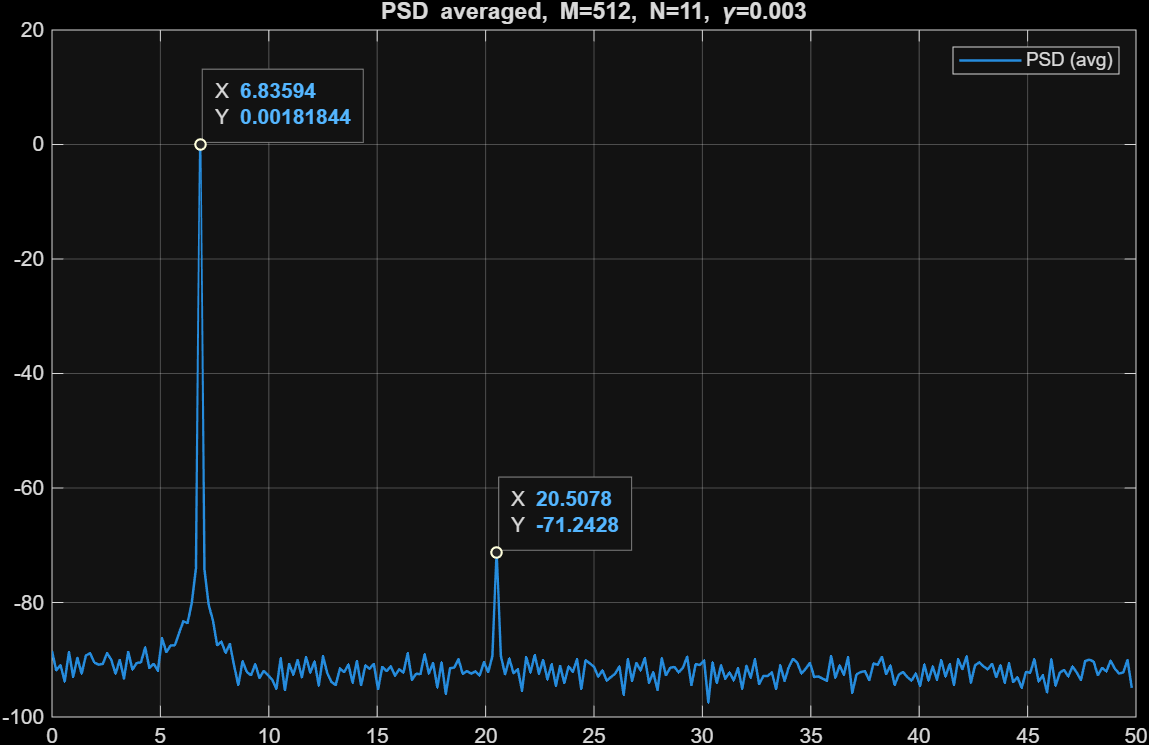
\includegraphics[width=1\textwidth]{img/task5_512.png}
    \caption{FFT with $M=512$, $N=11$, $\gamma=0.003$}
    \label{fig:task5_512}
\end{figure}

\vspace{1cm}
\textbf{Question: Using $M=2048$, repeat the previous step for $\gamma = 0.01$ and $0.1$. Are the spectral spurs located where you would expect?
}
\vspace{0.5cm}

From the FFT plots in Figures~\ref{fig:task5_y_0_01} and~\ref{fig:task5_y_0_1}, we can observe that as $\gamma$ increases, the amplitude of the distortion components (spurs) also increases.
For $\gamma = 0.01$, the spurs appear at the expected harmonic frequencies of the input tone, while for $\gamma = 0.1$ they become much more pronounced and clearly visible.

This confirms that the nonlinearity introduced by the companding function $g_\gamma(x)$ generates harmonic distortion.
The stronger the nonlinearity (larger $\gamma$), the greater the amplitude of these harmonics and the lower the SFDR.

\begin{figure}[H]
    \centering
    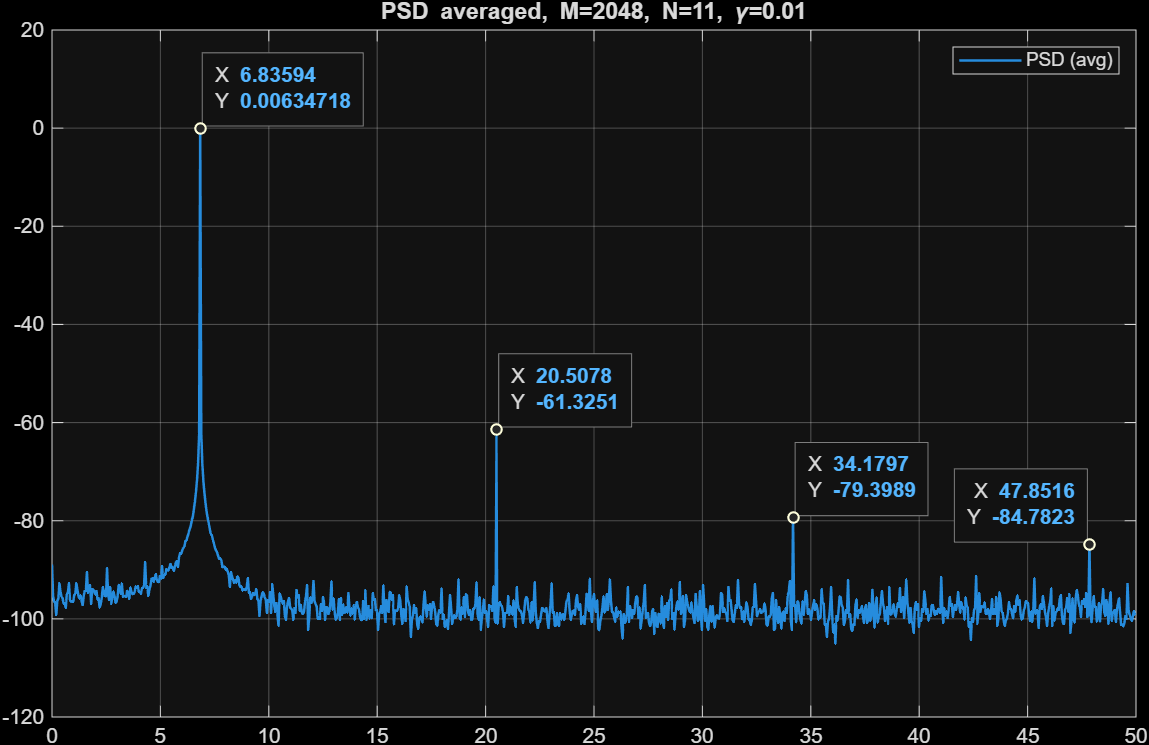
\includegraphics[width=1\textwidth]{img/task5_y_0_01.png}
    \caption{FFT with $M=2048$, $N=11$, $\gamma=0.01$}
    \label{fig:task5_y_0_01}
\end{figure}

\begin{figure}[H]
    \centering
    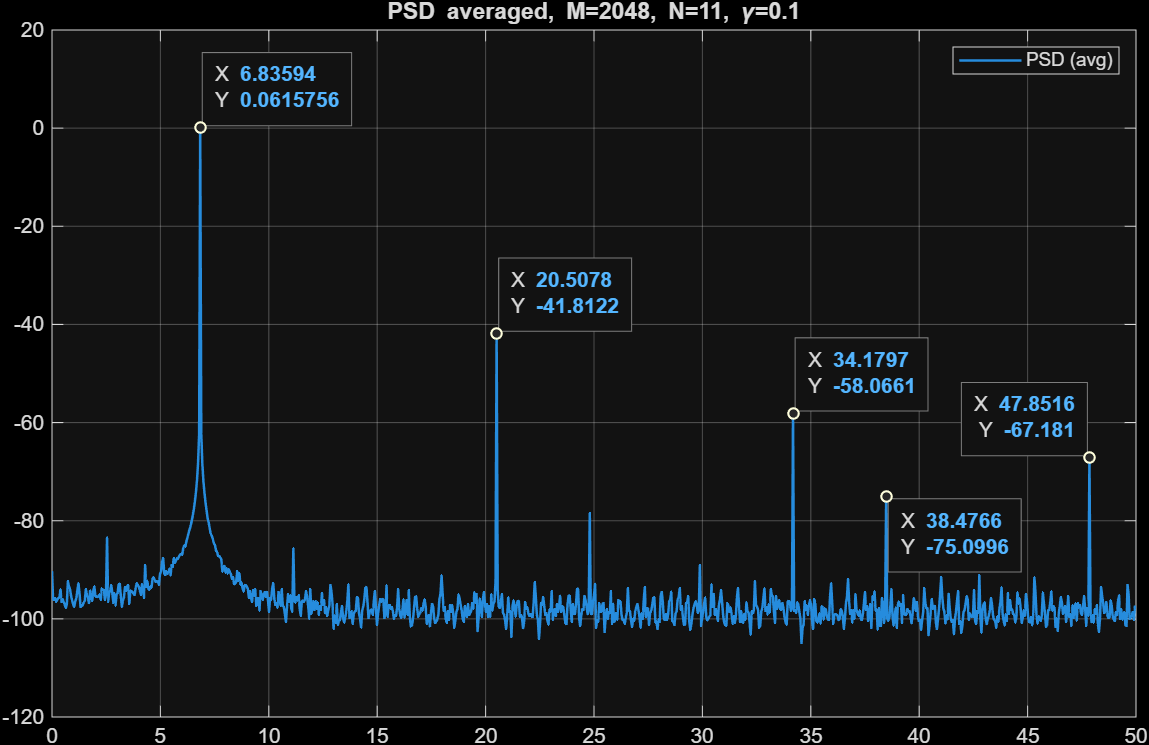
\includegraphics[width=1\textwidth]{img/task5_y_0_1.png}
    \caption{FFT with $M=2048$, $N=11$, $\gamma=0.1$}
    \label{fig:task5_y_0_1}
\end{figure}

\vspace{1cm}
\textbf{Question: Set now the amplitude to $\frac{\rm FS}{3}$. Using $M=2048$, measure the SFDR and express it in both dBFS and dBc for $\gamma=0.005$, $0.05$ and $0.1$. Will these values change if you repeat the analysis with $M=512$?
}
\vspace{0.5cm}

From Figure~\ref{fig:task5_5}, we can see that when the input amplitude is reduced to $\frac{\mathrm{FS}}{3}$, the fundamental tone decreases while the relative amplitude of the spurious components (spurs) remains almost unchanged.
This causes the SFDR values, both in dBFS and dBc, to be slightly worse than in the full-scale case.

As $\gamma$ increases, the nonlinearity becomes stronger and the harmonic distortion more evident, especially for $\gamma = 0.1$.
The comparison between $M = 2048$ and $M = 512$ shows that the FFT size does not significantly change the SFDR value; it only affects the frequency resolution, making the spectrum appear smoother and more detailed for higher $M$.

\begin{figure}[H]
  \centering
  % fila 1 (3 imágenes)
  \begin{subfigure}[t]{0.45\textwidth}
    \centering
    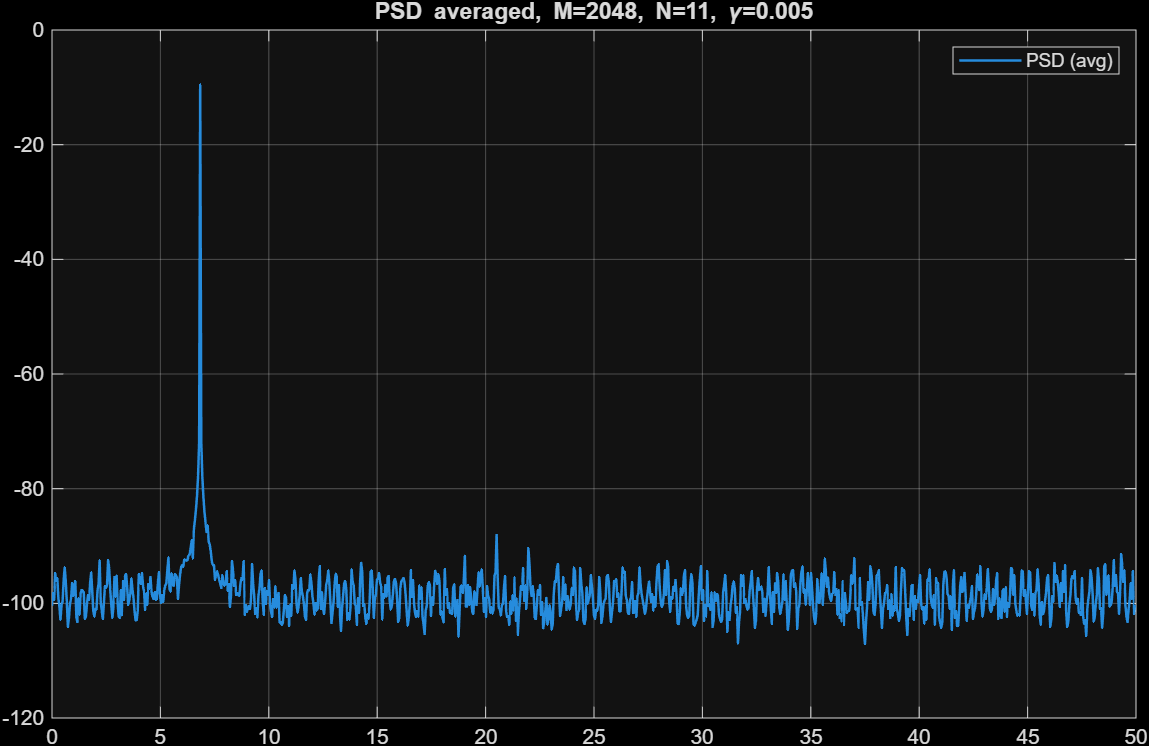
\includegraphics[width=\linewidth,height=0.28\textheight,keepaspectratio]{img/task5_5_1.png}
    \caption{FFT with $M=2048$, $N=11$, $\gamma=0.005$}
  \end{subfigure}\hfill
  \begin{subfigure}[t]{0.45\textwidth}
    \centering
    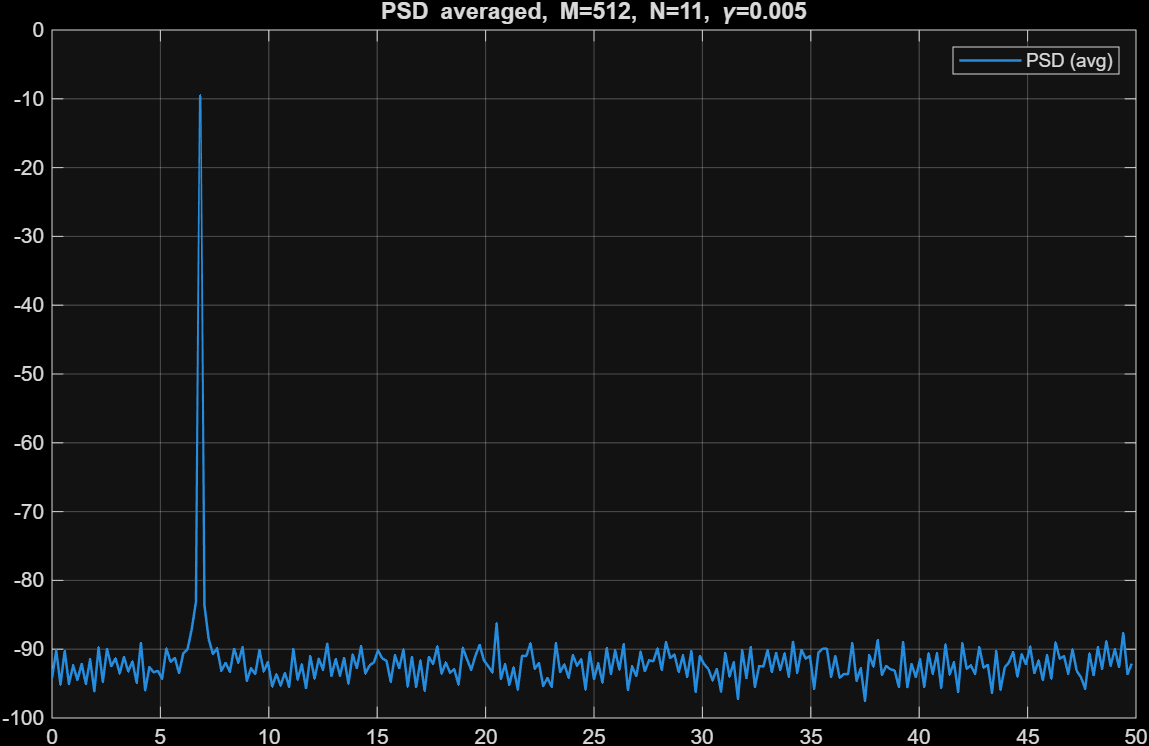
\includegraphics[width=\linewidth,height=0.28\textheight,keepaspectratio]{img/task5_5_4.png}
    \caption{FFT with $M=512$, $N=11$, $\gamma=0.005$}
  \end{subfigure}

  \vspace{1ex}

  \begin{subfigure}[t]{0.45\textwidth}
    \centering
    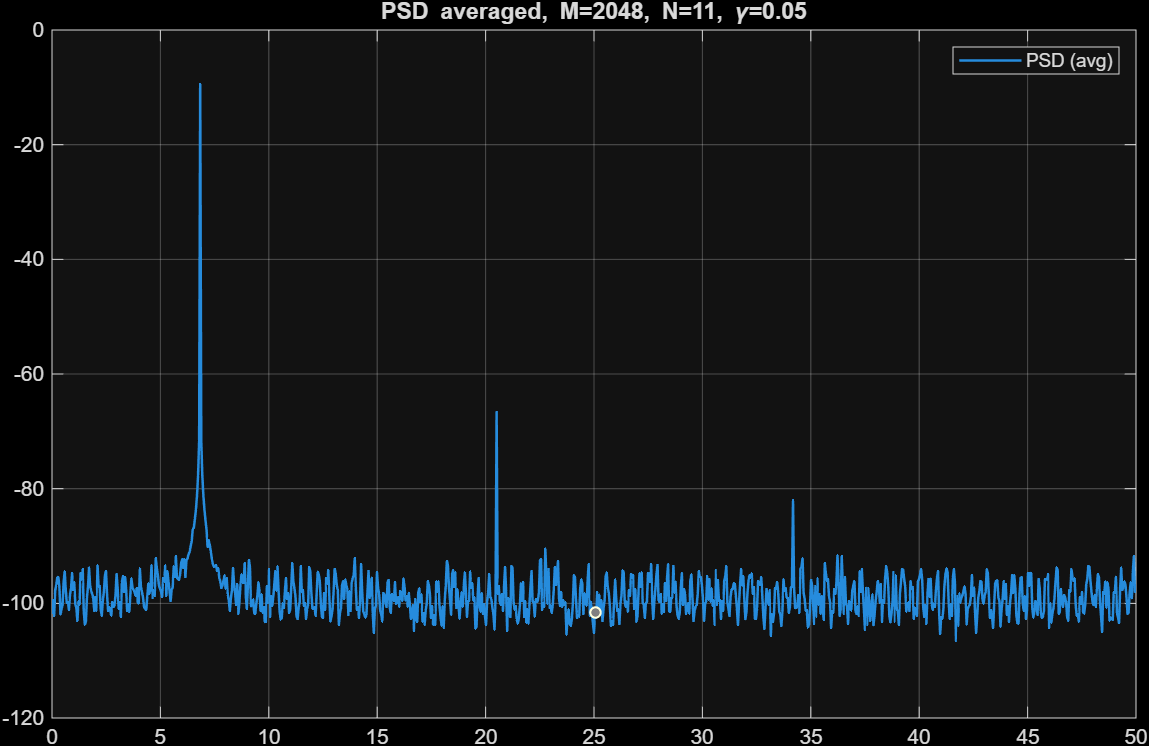
\includegraphics[width=\linewidth,height=0.28\textheight,keepaspectratio]{img/task5_5_2.png}
    \caption{FFT with $M=2048$, $N=11$, $\gamma=0.05$}
  \end{subfigure}\hfill
  \begin{subfigure}[t]{0.45\textwidth}
    \centering
    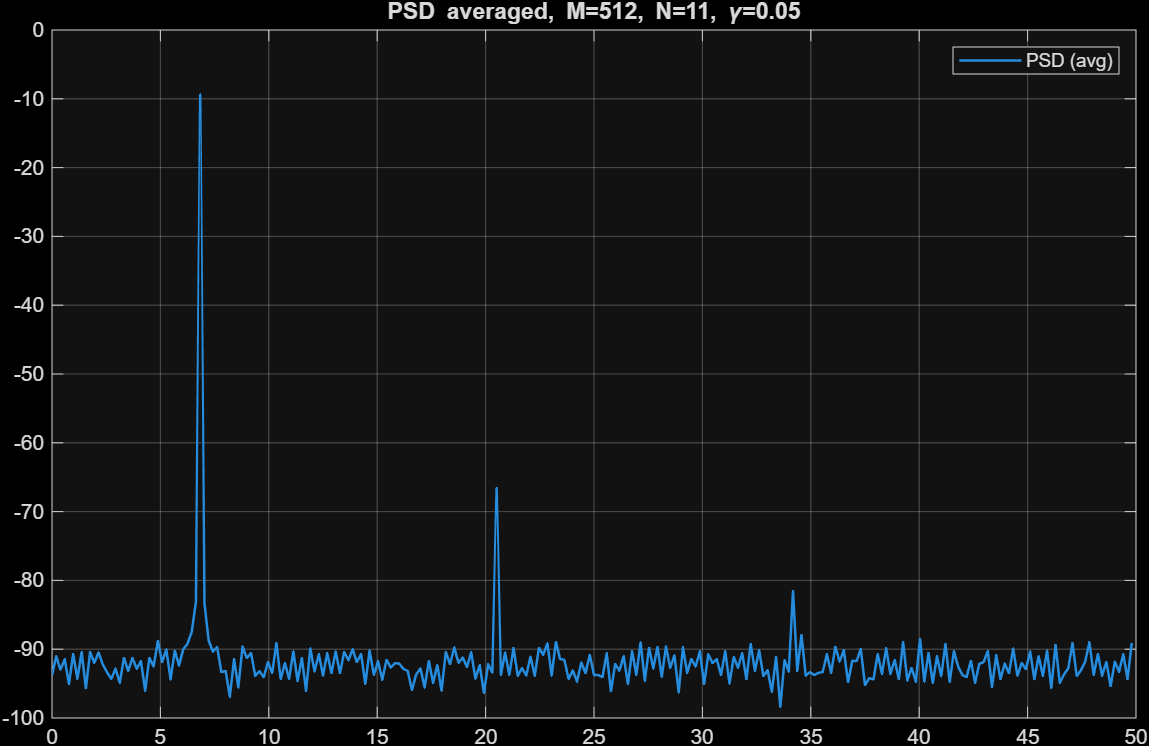
\includegraphics[width=\linewidth,height=0.28\textheight,keepaspectratio]{img/task5_5_5.png}
    \caption{FFT with $M=512$, $N=11$, $\gamma=0.05$}
  \end{subfigure}

  \vspace{1ex}

  \begin{subfigure}[t]{0.45\textwidth}
    \centering
    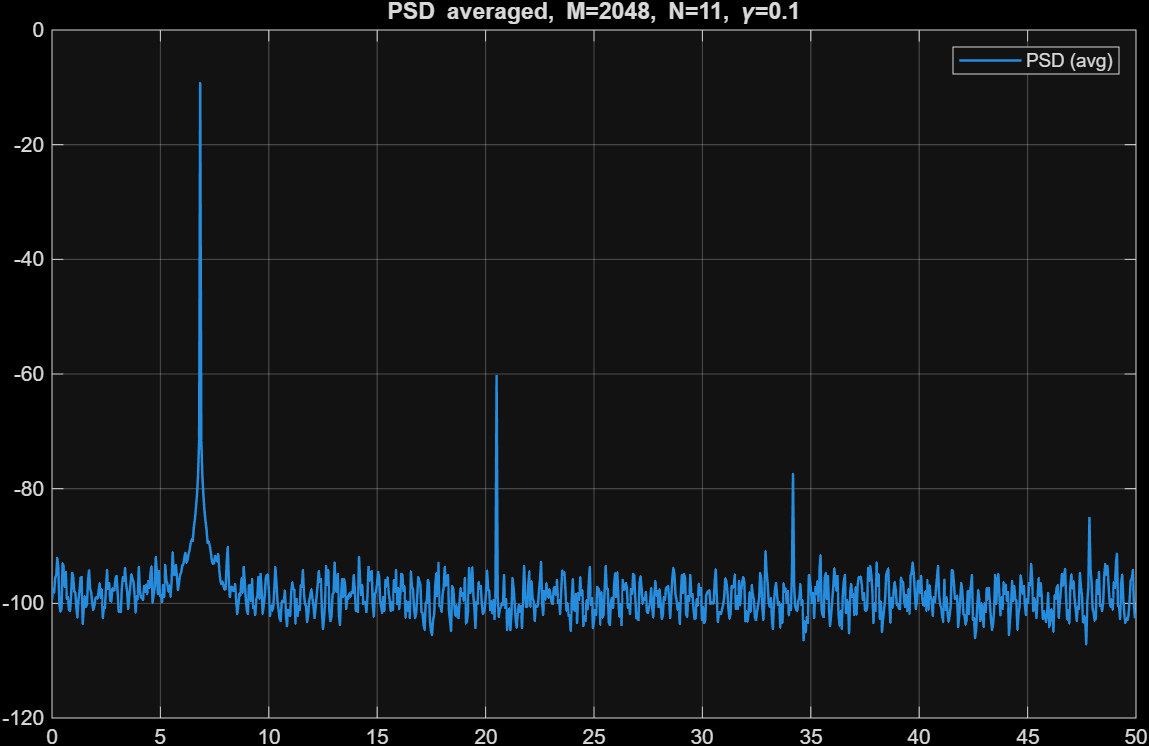
\includegraphics[width=\linewidth,height=0.28\textheight,keepaspectratio]{img/task5_5_3.png}
    \caption{FFT with $M=2048$, $N=11$, $\gamma=0.1$}
  \end{subfigure}\hfill
  \begin{subfigure}[t]{0.45\textwidth}
    \centering
    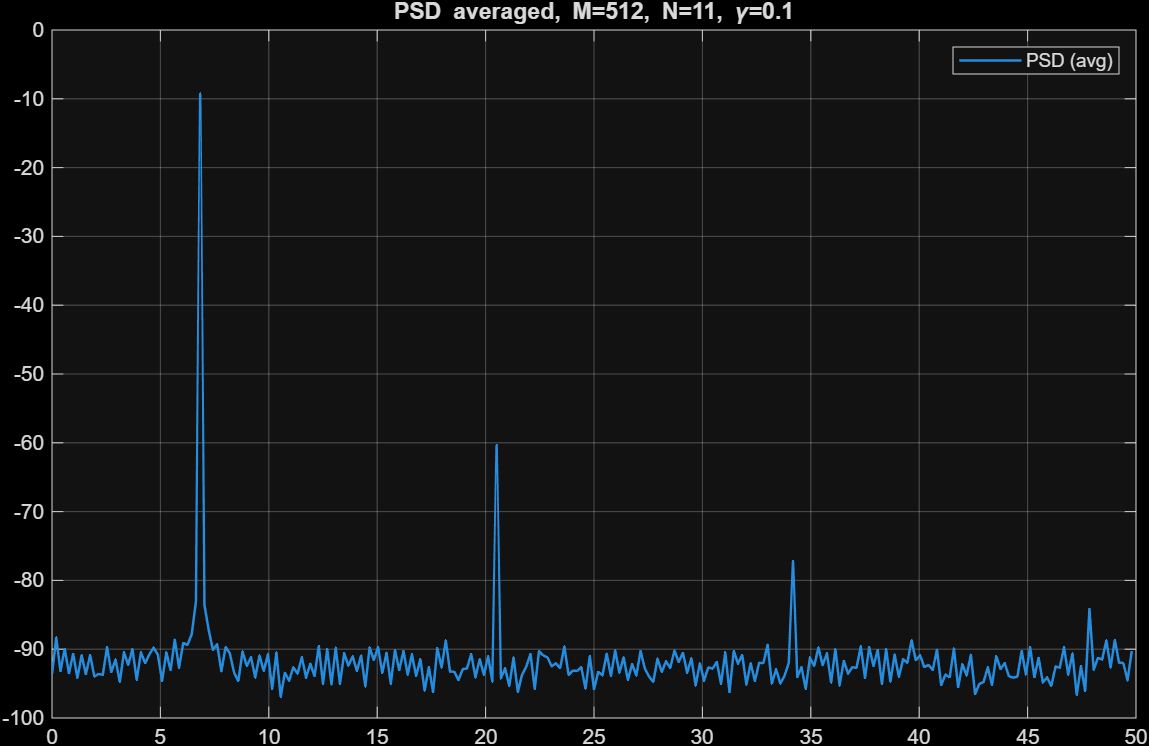
\includegraphics[width=\linewidth,height=0.28\textheight,keepaspectratio]{img/task5_5_6.png}
    \caption{FFT with $M=512$, $N=11$, $\gamma=0.1$}
  \end{subfigure}

  \caption{FFTs with different $M$ values, $N=11$, and varying $\gamma$.}
  \label{fig:task5_5}
\end{figure}

\vspace{1cm}
\textbf{Question: Consider now samples (at 100 MHz and with 11-bit resolution) of a sinusoid with frequency $3.3202$ MHz and amplitude $\frac{\rm FS}{2}$. Obtain the THD for this nonuniform ADC with $\gamma = 0.3$ under the IEEE 1241-2000 specification, expressed in both dB and percentage.
}
\vspace{0.5cm}

xd

